\documentclass{article}

% NeurIPS 2024 style (preprint: author-visible, no line numbers).
% Switch to \usepackage{neurips_2024} for anonymous submission,
% or \usepackage[final]{neurips_2024} for camera-ready copy.
\usepackage[preprint]{neurips_2024}

\usepackage[T1]{fontenc}
\usepackage[utf8]{inputenc}
\usepackage{amsmath,amssymb,amsthm}
\usepackage{booktabs}
\usepackage{graphicx}
\usepackage{xcolor}
\usepackage{array}
\usepackage{tabularx}
\usepackage{multirow}
\usepackage{enumitem}
\usepackage{microtype}
\usepackage{url}
\usepackage{hyperref}

\hypersetup{
  colorlinks=true,
  linkcolor=blue!50!black,
  citecolor=blue!50!black,
  urlcolor=blue!50!black,
  pdftitle={Preserving Task-Relevant Geometry in LLM Hidden States},
  pdfauthor={Tomohiko Nakamura}
}

\graphicspath{{figures/}}

\definecolor{confblue}{HTML}{0072B2}
\definecolor{explorange}{HTML}{D55E00}
\newcommand{\auroc}{\mathrm{AUROC}}
\newcommand{\propk}{\mathrm{PROP}\text{-}\kappa}
\newcommand{\bllen}{\mathrm{BL\text{-}LEN}}
\newcommand{\blnorm}{\mathrm{BL\text{-}NORM}}
\newcommand{\pca}{\mathrm{PCA}}
\newcommand{\CIint}[2]{[$#1$, $#2$]}
\newcommand{\exptag}{\textsc{exp--trj001}}

\title{Preserving Task-Relevant Geometry in {LLM} Hidden States:\\
Evidence That Variance-Maximizing {PCA} Can Obscure Hallucination Trajectory Signals}

\author{%
  Tomohiko Nakamura \\
  Gemmina Intelligence LLC
}

\begin{document}

\maketitle

\begin{abstract}
This study evaluates whether token-level hidden-state trajectories from selected layers of a large language model ({LLM}) can provide non-destructive signals for detecting response reliability and hedging/hallucination-related behavior~\citep{ji2023survey,azaria2023internal,farquhar2024semantic}. The study was conducted under a pre-registered protocol~\citep{nosek2018prereg,exptrj001plan} in which the primary confirmatory analysis used a $64$-dimensional principal component analysis ({PCA}) projection of the original $3584$-dimensional hidden states.

All five Layer~16 representations---{PCA} $64${D} ($0.7806$), {PC4}--{67} ($0.7969$), $\bllen$ ($0.8077$), raw $3584${D} $\propk$ ($0.8472$), and $\blnorm$ ($0.8588$)---are compared as \emph{paired} evaluations on the same $98$-prompt test inventory ($n=496$ eligible generations). Under the pre-registered {PCA} condition, $\propk$ failed the Gate~3 criterion for exceeding the response-length baseline ($\Delta=-0.0271$, $p=0.8685$; Gate~3: \textbf{fail}). Removing compression recovered $\auroc=0.8472$ versus $\bllen$ ($\Delta=+0.0395$, $95\%$~{CI} $[0.0114, 0.0726]$, $p=0.004$; exploratory). Discarding {PC1}--{3} ({PC4}--{67}) raised {AUROC} only to $0.7969$ ($\Delta=-0.0108$, $p=0.6935$). The hidden-state $L_2$-norm baseline $\blnorm$ is the strongest single predictor ($0.8588$, $95\%$~{CI} $[0.8239, 0.8903]$).

{PCA} diagnostics show that {PC1}--{3} capture $99.933\%$ of calibration variance, consistent with massive-activation dimensions monopolizing global variance in modern {LLMs}~\citep{sun2024massive}. Variance-maximizing {PCA} therefore collapses the state space to a very low effective rank and can discard directional trajectory geometry. The findings indicate that variance-preserving representation is not equivalent to signal-preserving representation for internal trajectory probing. The load-bearing paired contrast on this split is {PC4}--{67} versus {PCA} $64${D} ($\Delta=+0.0163$): discarding the three variance-dominant axes is not a sufficient repair.
\end{abstract}

\paragraph{Core thesis.}
The problem is not dimensionality reduction itself; it is reducing the wrong geometry. Variance-preserving dimensionality reduction is not necessarily signal-preserving dimensionality reduction for {LLM} internal-state trajectory analysis.

\paragraph{Study metadata.}
Experiment~\exptag{} / {EXP-2026-NVS-001}. Primary model: \texttt{Qwen/Qwen2.5-7B-Instruct}~\citep{qwen25,yang2024qwen2}. Evaluated layers: $8$, $16$, $24$. Hidden dimension $D=3584$. Primary confirmatory representation: $64${D} {PCA}. Paired exploratory and baseline conditions on the same $98$-prompt test set: raw $3584${D} trajectory features, {PC4}--{67}, $\bllen$, and $\blnorm$.

%======================================================================
\section{Introduction}
\label{sec:intro}

\subsection{Background and motivation}
\label{sec:intro-bg}

Large language models have demonstrated strong performance across a broad range of language and reasoning tasks, yet reliable estimation of whether a generated response is correct, supported, or hallucinated remains difficult~\citep{ji2023survey,huang2025survey}. Conventional evaluation often observes only the final generated text. Such output-level evaluation is useful, but it provides limited access to the internal dynamics by which a model arrives at an answer.

Hidden states provide a potential non-destructive observation channel into these internal dynamics~\citep{azaria2023internal,orgad2024llms,marks2024geometry,chen2024inside}. During autoregressive generation~\citep{vaswani2017}, the model produces a sequence of internal vector states associated with successive generated tokens. Instead of treating hidden states only as static feature vectors, they can be treated as a trajectory in a high-dimensional representational space~\citep{farquhar2024semantic}.

This study focuses on that trajectory perspective. The central question is not merely whether a hidden-state vector contains information related to response reliability, but whether \emph{the geometry and dynamics of the hidden-state trajectory} contain useful predictive information.

A practical obstacle arises immediately. Hidden states of modern {LLMs} are high dimensional. The model used in this study has a hidden dimension of $3584$. Storing, transporting, and repeatedly processing full trajectories can be computationally expensive. Dimensionality reduction is therefore attractive as an engineering strategy.

However, dimensionality reduction introduces a scientific question that is often treated as an implementation detail:

\begin{quote}
\centering\textbf{Which geometry should be preserved?}
\end{quote}

{PCA} is a standard answer when the objective is to preserve global variance~\citep{pearson1901,jolliffe2002,chvatal1983linear}. In modern {LLMs}, however, global variance is often dominated by a few massive-activation dimensions~\citep{sun2024massive}. Preserving global variance does not guarantee preserving the geometric structures that encode response reliability.

This study examines that distinction directly.

\subsection{The dimensionality-reduction problem}
\label{sec:intro-dr}

The primary confirmatory protocol specified a $64$-dimensional {PCA} projection. This creates a controlled comparison, executed on one paired $98$-prompt test inventory, among
(i)~uncompressed $3584${D} hidden-state trajectories,
(ii)~a variance-maximizing $64${D} {PCA} representation and the {PC4}--{67} subspace ablation,
(iii)~an output-level length baseline ($\bllen$), and
(iv)~a hidden-state magnitude baseline ($\blnorm$).

The underlying concern is that the principal directions that explain the greatest proportion of global variance may preferentially represent broad properties of language generation, while reliability-related dynamics may appear as smaller, localized, anisotropic, or otherwise non-dominant structures.

The point of the present study is not to argue that {PCA} is intrinsically defective. Rather, it asks whether \emph{variance preservation is sufficient for preserving the particular trajectory signal under study}.

\subsection{Research questions}
\label{sec:rqs}

\paragraph{{RQ1} --- Signal existence and localization.}
Can token-level hidden-state trajectories from the evaluated layers predict response reliability, and does their discriminative strength vary systematically across the evaluated layers?

\paragraph{{RQ2} --- {PCA} signal preservation.}
Does a variance-maximizing linear {PCA} projection to $64$ dimensions preserve trajectory-based discriminative signal sufficient to outperform the response-length baseline?

\paragraph{{RQ3} --- High-dimensional recovery.}
Can trajectory features derived from the uncompressed $3584$-dimensional hidden states recover predictive performance beyond the response-length baseline?

\subsection{Contributions}
\label{sec:contrib}

This study makes three primary contributions.

\begin{enumerate}[leftmargin=1.4em,itemsep=2pt]
\item \textbf{Transparent confirmatory negative result.}
The pre-registered $64${D} {PCA} condition did not satisfy the primary comparative Gate~3 criterion. The failure is reported directly rather than being replaced by a post hoc successful configuration~\citep{simmons2011false,nosek2018prereg}.

\item \textbf{Paired recovery of trajectory signal without variance-max {PCA}.}
On the same $98$-prompt test inventory, raw $3584${D} $\propk$ reached {AUROC} $0.8472$ ($\Delta=+0.0395$ vs.\ $\bllen$, $p=0.004$; exploratory). {PC4}--{67} improved on {PCA} $64${D} by only $\Delta=+0.0163$ and remained below $\bllen$. $\blnorm$ ($0.8588$) is reported in full on the identical $n=496$ eligible generations.

\item \textbf{Massive-activation account of variance collapse.}
{PC1}--{3} occupy $99.933\%$ of calibration variance. Following~\citet{sun2024massive}, we interpret this as massive-activation dimensions monopolizing global variance, so that variance-maximizing {PCA} distorts relative trajectory geometry rather than merely ``running out of dimensions.'' Intermediate-layer superiority of $\propk$ (Layer~$16$ vs.\ $8$/$24$) is reported as a trajectory-curvature reconfirmation of a known mid-depth probing pattern, not as a new localization claim.
\end{enumerate}

%======================================================================
\section{Background and related work}
\label{sec:bg}

\subsection{Internal-state probing and uncertainty}
\label{sec:rw-probe}

Probing internal representations for truthfulness and uncertainty has become a standard alternative to output-only evaluation~\citep{belinkov2019,alain2017probes,zou2023repeng}.
\citet{azaria2023internal} showed that linear classifiers on hidden states can detect whether a statement is likely true.
\citet{farquhar2024semantic} introduced semantic entropy to capture meaning-level uncertainty in generated sequences, rather than token-level predictive entropy alone.
Related internal detectors such as {INSIDE}~\citep{chen2024inside} and representation-geometry probes~\citep{orgad2024llms,marks2024geometry} measure structural properties of intermediate activations.
The present work builds on this line by treating the \emph{time series} of hidden states as a trajectory and scoring its discrete curvature $\kappa$, rather than a single static probe vector.

\subsection{Massive activations and variance dominance}
\label{sec:rw-massive}

\citet{sun2024massive} documented that modern {LLMs} exhibit \emph{massive activations}: a small subset of hidden dimensions with magnitudes orders of magnitude larger than the remainder, often nearly input-independent and tightly coupled to attention.
In any linear variance-based method such as {PCA}~\citep{pearson1901,hotelling1933,jolliffe2002}, those dimensions dominate the leading principal components.
On \texttt{Qwen2.5-7B-Instruct}, the frozen calibration diagnostic is consistent with that mechanism: {PC1}--{3} capture $99.933\%$ of token-level variance, and {PC1}--{64} capture $99.992\%$.
Variance-maximizing projection can therefore collapse $D=3584$ into an extremely low effective rank governed by activation \emph{magnitude}, suppressing the subtler directional transitions that trajectory $\kappa$ is designed to measure.

\subsection{Trajectory $\kappa$: cosine change and discrete curvature}
\label{sec:kappa}

Let $\mathbf{z}_t \in \mathbb{R}^{D}$ denote the (possibly {PCA}-projected) hidden state at generated-token index $t\in\{1,\ldots,T\}$ and selected layer $\ell$, with $D=3584$ in raw space and $D=64$ after the confirmatory projection.
Two geometric summaries of successive states are relevant.

\paragraph{Directional (cosine) transition.}
The one-step cosine change, evaluated after per-token $L_2$ normalization $\hat{\mathbf{z}}_t=\mathbf{z}_t/\lVert\mathbf{z}_t\rVert_2$, is
\begin{equation}
  \kappa^{\mathrm{cos}}_{t}
  \;=\;
  1
  -
  \hat{\mathbf{z}}_t^{\top}\hat{\mathbf{z}}_{t+1}
  \;=\;
  1
  -
  \frac{\mathbf{z}_t^{\top}\mathbf{z}_{t+1}}
       {\lVert\mathbf{z}_t\rVert_2\,\lVert\mathbf{z}_{t+1}\rVert_2},
  \qquad t=1,\ldots,T-1.
\label{eq:kappa-cos}
\end{equation}
Equation~\eqref{eq:kappa-cos} is a \emph{scale-invariant directional} statistic: it is unchanged under any per-token rescaling $\mathbf{z}_t\mapsto \alpha_t\mathbf{z}_t$ with $\alpha_t>0$. Gram curvature~\eqref{eq:kappa-curv} is \emph{not} scale-invariant (it scales as inverse length). Confirmatory $\propk$ remains the frozen Gram estimator; $\kappa^{\mathrm{cos}}$ is the diagnostic that isolates turning from magnitude. Spearman correlation of \texttt{kappa\_mean} with mean $\lVert\mathbf{z}_t\rVert_2$, $\kappa^{\mathrm{cos}}$ {AUROC} on $L_2$-normalized trajectories, and the residual of $\kappa$ after regression on norm are the empirical checks of this distinction (\texttt{scripts/run\_trj001\_reanalysis.py}, Task~B).

\paragraph{Frozen confirmatory curvature.}
The reported $\propk$ scores use the pre-registered discrete curvature of~\citet{exptrj001plan}, implemented in \texttt{src/compute\_kappa.py}. Parameterization is by token index, not arc length (an explicit, frozen choice: arc-length reparameterization would remove token-to-token speed variation). Central differences are
\begin{equation}
  \mathbf{v}_t
  \;=\;
  \frac{\mathbf{z}_{t+1}-\mathbf{z}_{t-1}}{2},
  \qquad
  \mathbf{a}_t
  \;=\;
  \mathbf{z}_{t+1}-2\mathbf{z}_t+\mathbf{z}_{t-1}.
\label{eq:va}
\end{equation}
With Gram matrix $G_t$ of $(\mathbf{v}_t,\mathbf{a}_t)$,
\begin{equation}
  \det G_t
  \;=\;
  \lVert\mathbf{v}_t\rVert_2^2\,\lVert\mathbf{a}_t\rVert_2^2
  -(\mathbf{v}_t^{\top}\mathbf{a}_t)^2,
  \qquad
  \kappa_t
  \;=\;
  \frac{\sqrt{\det G_t}}{\lVert\mathbf{v}_t\rVert_2^3+\varepsilon},
\label{eq:kappa-curv}
\end{equation}
where $\varepsilon=10^{-8}$ is frozen. Endpoints $t=1$ and $t=T$ are undefined by construction and are excluded. Sequences with $T<20$ are Class~E and are excluded from analysis.

From the valid scalar series $\{\kappa_t\}$, five length-normalized summaries form $\mathbf{x}_{\kappa}\in\mathbb{R}^{5}$:
mean, maximum, $95$th percentile, standard deviation, and {AUC} density $\frac{1}{T-2}\sum_t \kappa_t$
(\texttt{kappa\_mean}, \texttt{kappa\_max}, \texttt{kappa\_p95}, \texttt{kappa\_std}, \texttt{kappa\_auc\_density}).
The confirmatory feature set also includes \texttt{spike\_rate}$=(T-2)^{-1}\sum_t \mathbf{1}[\kappa_t>\theta]$, with $\theta$ the $90$th percentile of train-split $\kappa_t$. The raw $3584${D} ablation dropped \texttt{spike\_rate} because train-split raw states were unavailable to calibrate $\theta$; that condition difference is why {ABL-1} is exploratory. A matched $5$-feature {PCA} $64${D} probe (same summaries, no \texttt{spike\_rate}) is the confounder control for feature cardinality and is computed by the reanalysis script (Task~D).

\subsection{Classifier specification}
\label{sec:clf}

Every representation---$\propk$, $\propk+\mathrm{LEN}$, $\bllen$, and $\blnorm$---is scored by the same $L_2$-regularized logistic regression~\citep{exptrj001plan}.
Features are standardized with \texttt{sklearn.preprocessing.StandardScaler} fit on the training split only.
The inverse-regularization grid is
\begin{equation}
  C \in \{10^{-3},\,10^{-2},\,10^{-1},\,1,\,10,\,100\},
\end{equation}
selected by validation {AUROC} and then frozen for the test evaluation.
On Layer~16 the freeze record selected $C=0.1$ for $\propk$, $C=0.001$ for $\bllen$, and $C=100$ for $\blnorm$.
Test discrimination is {AUROC}~\citep{hanley1982,fawcett2006} with prompt-clustered bootstrap ($2{,}000$ resamples); {DeLong} tests are not used because the eight samples of one prompt are not independent~\citep{efron1993}.

\subsection{{PCA} versus task-relevant information}
\label{sec:bg-pca}

For a rank-$k$ projection $P_k$, the classical {PCA} objective is conceptually $\max_{P_k}\operatorname{Var}(P_k\mathbf{x})$ under orthogonality~\citep{pearson1901,jolliffe2002}.
That objective is reconstruction fidelity, not hallucination discrimination:
\begin{equation}
\boxed{\
  \text{high explained variance}
  \ \neq\
  \text{high task-relevant information}
\ }.
\label{eq:var-neq-signal}
\end{equation}

\paragraph{Observation / interpretation / hypothesis.}
On the paired Layer~16 test split,
$\auroc_{\mathrm{Raw}}=0.8472>\auroc_{\mathrm{PCA64}}=0.7806$,
with $\Delta_{\mathrm{PCA64\ vs\ }\bllen}=-0.0271$ ($p=0.8685$) versus
$\Delta_{\mathrm{Raw\ vs\ }\bllen}=+0.0395$ ($p=0.004$).
The evaluated {PCA} projection therefore does not preserve all discriminative trajectory information present in the raw states.
A candidate mechanism, not established as unique, is that task-relevant directional dynamics are misaligned with massive-activation axes selected by global variance~\citep{sun2024massive,park2024linear,elhage2022toy}.

%======================================================================
\section{Experimental protocol}
\label{sec:protocol}

\subsection{Model and inference environment}
\label{sec:env}

The frozen experimental environment records the configuration in Table~\ref{tab:env}. These values are recorded in the experimental freeze manifest~\citep{exptrj001freeze}. The model entry explicitly records the migration to {Qwen} from the previously considered {Llama} configuration. Inference used \texttt{vLLM}~\citep{kwon2023vllm}.

\begin{table}[t]
\centering
\caption{Frozen experimental environment (\texttt{results/env\_info.json}).}
\label{tab:env}
\small
\begin{tabular}{@{}ll@{}}
\toprule
Item & Value \\
\midrule
Model & \texttt{Qwen/Qwen2.5-7B-Instruct} \\
Model commit & \texttt{a09a35458c702b33eeacc393d103063234e8bc28} \\
vLLM & \texttt{0.29.0} \\
{CUDA} / driver & {CUDA} $13.0$ \\
Torch & \texttt{2.13.0+cu130} \\
{GPU} & {NVIDIA A40} \\
Python & $3.11.10$ \\
Hidden dimension & $3584$ \\
\bottomrule
\end{tabular}
\end{table}

\subsection{Dataset construction and filtering}
\label{sec:data}

The experiment uses Type~A, Type~B, and calibration prompt groups. Phase~1 included $1{,}000$ Type~A prompts and $8$ samples per prompt, producing $8{,}000$ generations in the pilot stage. The manifest records a mixed-prompt rate of $0.599$ and an observed mixed-positive rate of $0.471$.

The Phase~2 collection consisted of
\begin{equation}
  493\ \text{prompts}\times 8\ \text{samples}=3{,}944\ \text{generations}.
\end{equation}
The recorded label composition is given in Table~\ref{tab:labels}. After mixed-prompt filtering, $299$ prompts and $2{,}392$ samples remained. Binary targets map \texttt{type\_a\_positive} to $y=1$ and hedging/abstention (\texttt{type\_d\_hedge}, \texttt{type\_c\_abstain}) to $y=0$; the classifiers therefore score reliability versus hedging propensity rather than unhedged factual error alone.

Eligibility is evaluated at the \emph{prompt-cluster} level: a prompt is retained if and only if its eight generations meet the mixed-response criterion, so no partial clusters enter Phase~3~\citep{exptrj001plan}. Prompts were then partitioned at the prompt level into train $296$, validation $99$, and test $98$ (\texttt{configs/data\_splits.json}).

\paragraph{Paired evaluation set.}
All Layer~16 comparisons among raw $3584${D}, {PCA} $64${D}, {PC4}--{67}, $\bllen$, and $\blnorm$ are executed on this \emph{same} $98$-prompt test inventory. The freeze record reports $n_{\mathrm{test}}=496$ eligible generations after Class~E ($T<20$) exclusion ($98\times 8=784$ generations; $288$ excluded). $\bllen$ and $\blnorm$ are not scored on a different or larger set: they are strictly paired with the trajectory methods on these $496$ rows. This pairing removes inventory composition as a confounder: differences are attributable to representation, not to a changing prompt set. Label composition of the $288$ Class~E rows, and {AUROC} rank stability under $T\ge 10,15,20,30$, are defined by the reanalysis script and require the freeze trajectory store.

Type~A factual prompts are collision-checked with the {Wikipedia} {MediaWiki} \texttt{action=query} {API} using the \texttt{missing} flag; no second web-search backend is used (Appendix~\ref{app:filtering}).

\begin{table}[t]
\centering
\caption{Phase~2 label composition.}
\label{tab:labels}
\small
\begin{tabular}{@{}lr@{}}
\toprule
Label & Count \\
\midrule
\texttt{type\_a\_positive} & $2{,}191$ \\
\texttt{type\_d\_hedge} & $1{,}616$ \\
\texttt{type\_c\_abstain} & $137$ \\
\midrule
Total & $\mathbf{3{,}944}$ \\
\bottomrule
\end{tabular}
\end{table}

\subsection{Hidden-state extraction}
\label{sec:extract}

Hidden states are collected at the evaluated layers: Layer~8, Layer~16, and Layer~24.
Each token-level state has dimensionality $3584$ before projection.
The experiment retains both the lower-dimensional {PCA} trajectory representation and, for the designated ablation subset, the original high-dimensional hidden states.

The manifest records $98$ of $200$ originally targeted ablation prompts as available and retains that shortfall in \texttt{configs/ablation\_prompt\_ids.json} rather than silently replacing it. Those $98$ prompts \emph{are} the paired test inventory used for every Layer~16 representation below.

\begin{figure}[t]
\centering
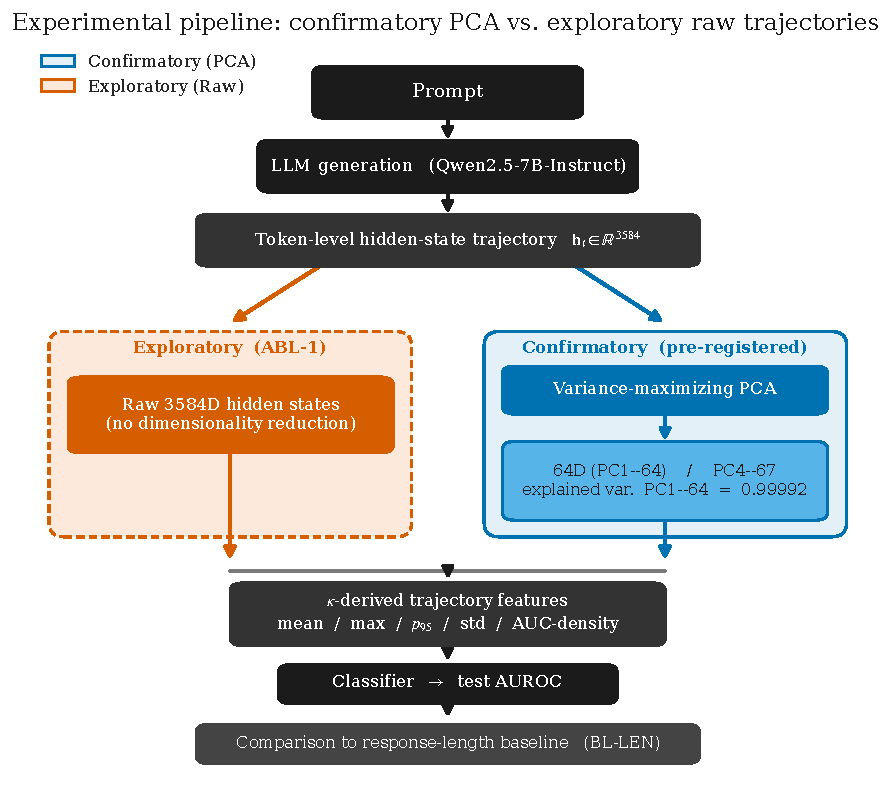
\includegraphics[width=\linewidth]{fig1_pipeline.pdf}
\caption{Experimental pipeline. Confirmatory analysis projects token-level hidden states with variance-maximizing {PCA} before $\kappa$-feature construction. The exploratory {ABL-1} branch derives the same curvature statistics from uncompressed $3584${D} states. Both branches, together with $\bllen$ and $\blnorm$, are scored by the same $L_2$-regularized logistic regression on the paired $98$-prompt test set.}
\label{fig:pipeline}
\end{figure}

\subsection{{PCA} configuration}
\label{sec:pca-cfg}

The frozen artifact set contains a {PCA} projection matrix with shape
\begin{equation}
  3584\times 128.
\end{equation}
The {PCA} diagnostics are reported in Table~\ref{tab:pca-diag}. These values show that the evaluated {PCA} representation retains extremely high global explained variance while still failing to demonstrate superiority over the response-length baseline in the primary comparative test.

The present study therefore treats explained variance as a representation diagnostic rather than as evidence of downstream task-signal preservation.

\begin{table}[t]
\centering
\caption{{PCA} diagnostics (Phase~0, Qwen2.5-7B-Instruct).}
\label{tab:pca-diag}
\small
\begin{tabular}{@{}lr@{}}
\toprule
Diagnostic & Value \\
\midrule
{PC1}--{64} cumulative explained variance & $0.99992$ \\
{PC1}--{128} cumulative explained variance & $0.99996$ \\
{PC1}--{3} cumulative explained variance & $0.99933$ \\
Number of calibration tokens & $8{,}357$ \\
\bottomrule
\end{tabular}
\end{table}

\subsection{Representations and baselines}
\label{sec:baselines}

Five Layer~16 representations are scored on the paired test set (Figure~\ref{fig:pipeline}):
\begin{enumerate}[leftmargin=1.4em,itemsep=2pt]
\item \textbf{{PCA} $64${D} (confirmatory).}
Centered hidden states are projected onto {PC1}--{64} (fit on $8{,}357$ calibration tokens) before $\kappa$ extraction.
\item \textbf{{PC4}--{67} (subspace ablation).}
The same protocol on principal components $4$ through $67$, discarding {PC1}--{3}.
\item \textbf{Raw $3584${D} (exploratory).}
$\kappa$ features from uncompressed hidden vectors; \texttt{spike\_rate} omitted (no train-split raw $\theta$).
\item \textbf{$\bllen$ (output baseline).}
Response token length $T$ only. This is the pre-registered Gate~3 comparator.
\item \textbf{$\blnorm$ (magnitude baseline).}
Statistics of $\lVert\mathbf{z}_t\rVert_2$ along the trajectory (mean, maximum, standard deviation). Reported in full: it is a first-class baseline, not a suppressed comparator.
\end{enumerate}

{PCA} diagnostics (Table~\ref{tab:pca-diag}) show that the confirmatory $64${D} representation retains $99.992\%$ of global variance while still failing Gate~3. Explained variance is therefore a representation diagnostic, not evidence of task-signal preservation.

\subsection{Statistical evaluation}
\label{sec:stats}

The primary discrimination metric is test {AUROC}.
For comparisons against $\bllen$, the analysis reports
(i)~the {AUROC} difference $\Delta$,
(ii)~a bootstrap $95\%$ confidence interval~\citep{efron1993}, and
(iii)~the corresponding empirical comparison $p$-value reported by the frozen analysis.

Layer-family comparisons use Holm correction~\citep{holm1979} across the specified pairwise comparisons.

The study maintains a distinction between
\begin{enumerate}[leftmargin=1.4em]
\item \textbf{confirmatory analysis}, defined by the pre-registered protocol; and
\item \textbf{exploratory analysis}, performed after the pre-registered outcome was obtained.
\end{enumerate}
This distinction is maintained throughout the Results and Discussion sections.

\subsection{Pre-registration and freeze protocol}
\label{sec:freeze}

The freeze manifest defines a strict rule~\citep{exptrj001freeze}:
\begin{quote}
Data generated before the freeze is not to be adopted as an experimental result.
\end{quote}
The manifest also lists hashes for the experimental plan, {PCA} matrix, centering vector, prompt inventories, label logic, generation configuration, masking procedure, and Type~B reference assets.

The current uploaded manifest still shows the freeze timestamp, freeze commit, and approver fields as unfilled. The document also specifies that the freeze becomes formally established when all hash fields are complete and the \texttt{v1.4-frozen} tag has been applied. This administrative state must be checked and finalized before submission as a formally frozen study.

%======================================================================
\section{Results}
\label{sec:results}

\subsection{Confirmatory Gate~3 evaluation ({RQ2})}
\label{sec:act1}

The primary confirmatory evaluation used {PCA} $64${D} $\propk$ at Layer~16 on the paired $98$-prompt test set:
\begin{equation}
  \auroc_{\propk}=0.7806,
  \qquad
  \auroc_{\bllen}=0.8077,
\end{equation}
with $\Delta=-0.0271$, $95\%$~{CI} $[-0.0727,\ 0.0190]$, $p=0.8685$.
Gate~3 condition~1 ({AUROC}$>0.5$) passed; condition~2 (exceed $\bllen$) failed:
\begin{equation}
\boxed{\ \text{Gate 3 = FAIL}\ }.
\label{eq:gate3}
\end{equation}
This negative result is the principal confirmatory finding. It does \emph{not} imply that hidden-state trajectories contain no useful information; it establishes only that the evaluated {PCA} trajectory representation did not beat $\bllen$ under the pre-registered criterion.

\subsection{Layer localization ({RQ1})}
\label{sec:act2}

Confirmatory $\propk$ {AUROC} varies across the three sampled layers (Table~\ref{tab:layer}, Figure~\ref{fig:layer}): $0.7090$ at Layer~8, $0.7806$ at Layer~16, and $0.7167$ at Layer~24.
Holm-corrected pairwise tests~\citep{holm1979} give Layer~16 vs.\ Layer~8 $\Delta=+0.0717$ ($95\%$~{CI} $[0.0359, 0.1080]$, $p<0.001$) and Layer~16 vs.\ Layer~24 $\Delta=+0.0639$ ($95\%$~{CI} $[0.0368, 0.0944]$, $p<0.001$).
This is localization \emph{within the evaluated set}, not a claim that Layer~16 is globally optimal.
When $\propk$ is concatenated with length, Layer~24 reaches $0.8314$ versus Layer~16's $0.8293$, indicating complementary sequence-length information in deeper layers.

\begin{table}[t]
\centering
\caption{Layer-wise confirmatory $\propk$ test {AUROC} with $95\%$ bootstrap confidence intervals.}
\label{tab:layer}
\small
\begin{tabular}{@{}crr@{}}
\toprule
Layer & $\propk$ {AUROC} & $95\%$ {CI} \\
\midrule
$8$  & $0.7090$ & $[0.6554,\ 0.7599]$ \\
$16$ & $\mathbf{0.7806}$ & $[0.7298,\ 0.8232]$ \\
$24$ & $0.7167$ & $[0.6570,\ 0.7693]$ \\
\bottomrule
\end{tabular}
\end{table}

\begin{figure}[t]
\centering
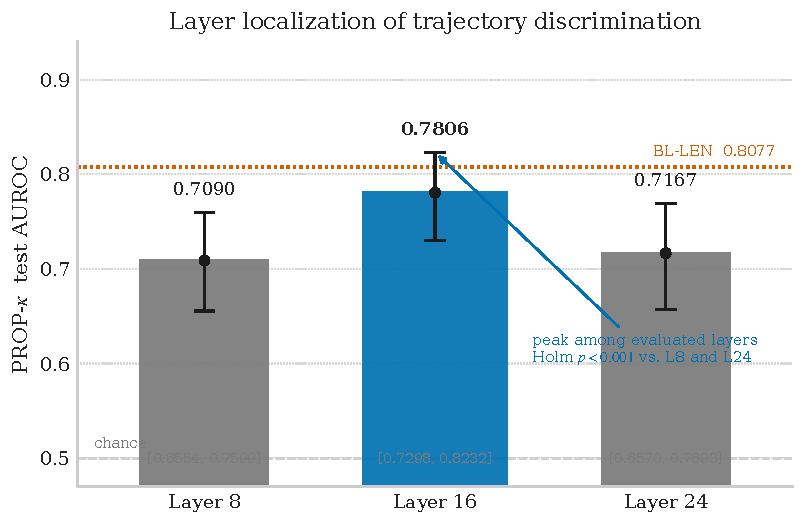
\includegraphics[width=\linewidth]{fig2_layer_auroc.pdf}
\caption{Layer localization of $\propk$ discrimination at Layers~$8$, $16$, and $24$, with bootstrap $95\%$ confidence intervals. Layer~16 is the peak among the evaluated layers. The dashed line marks $\bllen=0.8077$.}
\label{fig:layer}
\end{figure}

\subsection{Paired comparison of five representations ({RQ3})}
\label{sec:act3}

Table~\ref{tab:hero} and Figure~\ref{fig:hero} report every Layer~16 condition on the \emph{same} $98$-prompt test set. No comparator is omitted.

\begin{table}[t]
\centering
\caption{Paired Layer~16 comparison on the $98$-prompt test inventory ($n=496$). $\Delta$ and $p$ versus $\bllen$ are cluster-bootstrap estimates from the freeze record where available. $\blnorm$ $\Delta$ is the difference of point estimates; its {AUROC} {CI} lies entirely above the $\bllen$ point estimate.}
\label{tab:hero}
\small
\setlength{\tabcolsep}{3.5pt}
\begin{tabular}{@{}lrrll@{}}
\toprule
Representation & {AUROC} & $\Delta$ vs.\ $\bllen$ & $p$ & $95\%$ {CI} \\
\midrule
{PCA} $64${D} (confirmatory) & $0.7806$ & $-0.0271$ & $0.8685$ & $[0.7298,\ 0.8232]$ \\
{PC4}--{67} (ablation) & $0.7969$ & $-0.0108$ & $0.6935$ & $[0.7498,\ 0.8390]$ \\
$\bllen$ (output baseline) & $0.8077$ & --- & --- & $[0.7632,\ 0.8475]$ \\
Raw $3584${D} $\propk$ (exploratory) & $0.8472$ & $+0.0395$ & $0.004$ & $[0.8060,\ 0.8824]$ \\
$\blnorm$ (magnitude baseline) & $\mathbf{0.8588}$ & $+0.0511$ & --- & $[0.8239,\ 0.8903]$ \\
\bottomrule
\end{tabular}
\end{table}

\begin{figure}[t]
\centering
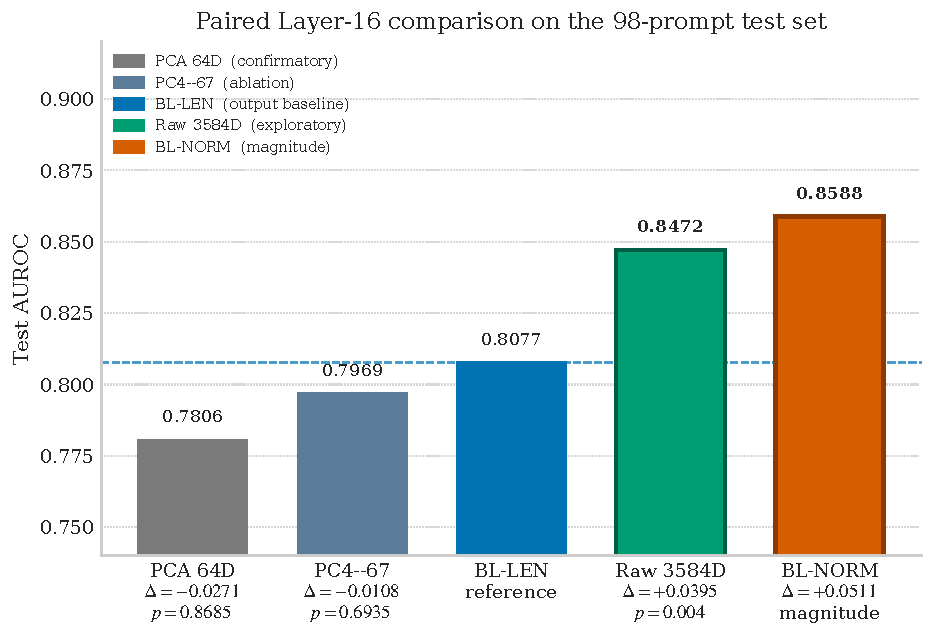
\includegraphics[width=\linewidth]{fig3_hero_comparison.pdf}
\caption{Paired Layer~16 test {AUROC} on the $98$-prompt set: {PCA} $64${D} ($0.7806$), {PC4}--{67} ($0.7969$), $\bllen$ ($0.8077$), raw $3584${D} ($0.8472$), and $\blnorm$ ($0.8588$). $\blnorm$ and {PC4}--{67} are reported in full. Raw vs.\ $\bllen$ is exploratory ($p=0.004$).}
\label{fig:hero}
\end{figure}

\paragraph{Raw $3584${D}.}
Removing {PCA} yields exploratory $\auroc=0.8472$ ($\Delta=+0.0395$ vs.\ $\bllen$, $p=0.004$). This is not a confirmatory Gate~3 success.

\paragraph{{PC4}--{67}.}
Discarding {PC1}--{3} improves on {PCA} $64${D} by $\Delta=+0.0163$ but remains below $\bllen$ ($0.7969$, $p=0.6935$ vs.\ $\bllen$). Leading-component removal is therefore not a sufficient fix.

\paragraph{$\blnorm$.}
Mean hidden-state $L_2$ norm is the strongest single predictor ($0.8588$; {CI} lower bound $0.8239>\auroc_{\bllen}$). Magnitude and directional $\kappa$ are complementary quantities; a joint model is not claimed here because a frozen combined AUROC is not in the Phase~3 record.

The ordering on this split is
\begin{equation}
\boxed{\
  \blnorm
  \ \ge\
  \text{raw }3584\text{D }
  \ >\
  \bllen
  \ >\
  \text{{PC4--}67}
  \ >\
  \text{{PCA }64\text{D}}
\ }.
\label{eq:ordering}
\end{equation}

%======================================================================
\section{Discussion}
\label{sec:disc}

\subsection{Massive-activation dominance of global variance}
\label{sec:disc-var}

The result is not that {PCA} is intrinsically unsuitable for {LLM} analysis. It is that two objectives need not share axes (Figure~\ref{fig:geometry}): variance/reconstruction versus reliability discrimination.

On Qwen2.5-7B, {PC1}--{3} explain $99.933\%$ of calibration variance and {PC1}--{64} explain $99.992\%$. Following~\citet{sun2024massive}, we interpret this spectrum as massive-activation dimensions monopolizing global variance. Variance-maximizing {PCA} then collapses $D=3584$ into a near-rank-$3$ magnitude subspace and can discard directional $\kappa$ dynamics.

This is not a claim that $64$ dimensions are numerically insufficient. Discrete curvature $\kappa_t$ is a property of the osculating plane spanned by $(\mathbf{v}_t,\mathbf{a}_t)$: the Gram determinant in~\eqref{eq:kappa-curv} is the squared area of that parallelogram, and $\kappa_t$ is unchanged if the trajectory is isometrically embedded in any ambient dimension $D'\ge 2$. Extra coordinates that are constant, or that merely rescale the same plane, cannot increase the intrinsic curvature. What {PCA} can do---and what the paired {PC4}--{67} increment of only $+0.0163$ is consistent with---is \emph{rotate and anisotropically rescale relative token placement} so that the projected curve is a distorted image of the original. The defect is distortion of relative configuration under a variance-max objective, not a missing-dimension budget.

That interpretation remains a mechanism \emph{hypothesis}: the experiment shows signal loss under this projection, not a unique localization of the lost bits in the discarded $0.008\%$ of variance.
The same magnitude geometry that dominates {PCA} is layer-dependent as a predictor: $\blnorm$ falls from $0.8588$ at Layer~$16$ to $0.7158$ at Layer~$24$, consistent with massive-activation structure changing near the output.
\begin{equation}
\boxed{\
  \text{high explained variance}
  \ \not\Rightarrow\
  \text{high task-relevant information}
\ }.
\label{eq:notimplies}
\end{equation}

\begin{figure}[t]
\centering
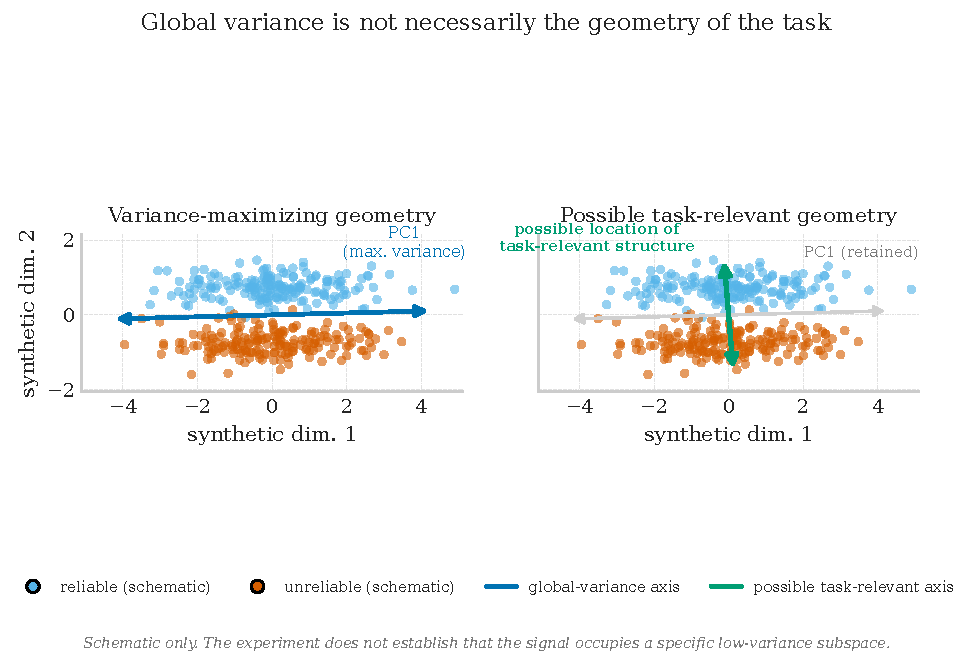
\includegraphics[width=\linewidth]{fig4_geometry.pdf}
\caption{Schematic: global-variance {PCA} axes versus \emph{possible} task-relevant structure. The diagram does not claim that the reliability signal occupies a proven low-variance subspace.}
\label{fig:geometry}
\end{figure}

\subsection{Facing $\blnorm$ as a first-class baseline}
\label{sec:disc-blnorm}

$\blnorm$ is the strongest individual score on the paired split ($0.8588$). Hiding it would invite the charge that a stronger internal baseline was suppressed. The result is scientifically informative: hedging/reliability is tightly coupled to activation \emph{magnitude}, exactly the geometry that massive activations and leading PCs occupy~\citep{sun2024massive}. Raw $\kappa$ ($0.8472$) is a directional statistic; $\blnorm$ is a magnitude statistic. They are not interchangeable, and Gate~3 remains defined against $\bllen$ because that was the pre-registered output-level comparator. A joint $\kappa$+norm model is left to follow-up work.

\subsection{Facing {PC4}--{67}}
\label{sec:disc-abl2}

{PC4}--{67} tests the story that {PC1}--{3} are the only nuisance directions. The paired gain over {PCA} $64${D} is small ($+0.0163$) and {PC4}--{67} still fails to beat $\bllen$ ($0.7969$ vs.\ $0.8077$, $p=0.6935$). Removing the massive-activation axes is therefore not sufficient to recover the raw-space $\kappa$ signal ($0.8472$). Residual explanations---nonlinear structure, local anisotropy, weak distributed directions---remain open~\citep{elhage2022toy,gurnee2023finding}.

\subsection{The central thesis}
\label{sec:disc-thesis}

The study therefore proposes the following design principle:
\begin{quote}
\textbf{The problem is not dimensionality reduction itself; it is reducing the wrong geometry.}
\end{quote}
A practical consequence is that future projection methods should be evaluated against two different criteria:
(i)~\textbf{representation preservation} and
(ii)~\textbf{task-signal preservation}.
A projection can score extremely well on the first and poorly on the second.
The present study provides evidence that this distinction matters for {LLM} hidden-state trajectory analysis.

\subsection{Engineering implications}
\label{sec:disc-eng}

The results matter beyond this particular experiment because high-dimensional hidden states are expensive to retain and process.
A future real-time system may need to transform
\begin{equation}
  3584\mathrm{D}\ \rightarrow\ 16\mathrm{D}\text{--}64\mathrm{D}
\end{equation}
while preserving the trajectory signal relevant to confidence or reliability estimation~\citep{kadavath2022,farquhar2024semantic}.

The implication is not that raw $3584${D} representations should always be retained in production. The more useful engineering question is:
\begin{quote}
\textbf{Can a compact learned geometry preserve the same task-relevant structure that the raw representation contains?}
\end{quote}
This motivates task-aware projection rather than variance-only compression.

\subsection{Limitations}
\label{sec:limits}

\subsubsection{Exploratory status of {ABL-1}}
Raw $3584${D} $\propk$ was obtained after the confirmatory outcome and dropped \texttt{spike\_rate}; it is exploratory.

\subsubsection{Target definition}
Binary labels map factual-positive versus hedge/abstain. The classifiers therefore probe hedging propensity, not unhedged factual hallucination alone.

\subsubsection{Limited layer sampling}
Only Layers~$8$, $16$, and $24$ were evaluated.

\subsubsection{Limited ablation inventory}
$98$ of $200$ designated ablation prompts were available; that shortfall is retained.

\subsubsection{Single-model evaluation}
Results are for \texttt{Qwen/Qwen2.5-7B-Instruct} only.

\subsubsection{Mechanism not identified}
Massive-activation dominance of {PC1}--{3} is a supported interpretation, not a unique geometric localization of the lost $\kappa$ signal.

%======================================================================
\section{Conclusions and future work}
\label{sec:concl}

\subsection{Conclusion}
\label{sec:concl-main}

This study began with a pre-registered hypothesis concerning whether a $64${D} {PCA} representation of {LLM} hidden-state trajectories could exceed a response-length baseline in hallucination/reliability discrimination.

The primary confirmatory analysis did not meet the Gate~3 criterion ($\auroc_{\mathrm{PCA64}}=0.7806<\auroc_{\bllen}=0.8077$, $\Delta=-0.0271$, $p=0.8685$).
On the same $98$-prompt test set, {PC4}--{67} reached only $0.7969$, raw $3584${D} $\propk$ reached $0.8472$ ($p=0.004$ vs.\ $\bllen$; exploratory), and $\blnorm$ reached $0.8588$.
{PC1}--{3} occupy $99.933\%$ of calibration variance, consistent with massive-activation monopoly of global variance~\citep{sun2024massive}.

The resulting scientific interpretation is deliberately narrower than a claim that {PCA} is universally harmful:
\begin{quote}
\textbf{The evaluated variance-maximizing {PCA} projection did not preserve all of the task-relevant trajectory signal available in the raw hidden-state representation.}
\end{quote}
This supports the broader design principle
\begin{equation}
\boxed{\
  \text{variance-preserving reduction}
  \ \neq\
  \text{signal-preserving reduction}
\ }
\label{eq:final-box}
\end{equation}
and motivates the search for projection methods that explicitly preserve task-relevant geometry.

\subsection{Future directions}
\label{sec:future}

\subsubsection{Geometry-preserving supervised projection}
The next experimental stage should construct a learned projection
\begin{equation}
  \mathbb{R}^{3584}\ \rightarrow\ \mathbb{R}^{16\text{--}64}
\end{equation}
that optimizes task-relevant structure rather than global variance alone (follow-up experiment {TRJ002a}).
Candidate approaches include supervised linear projection, supervised autoencoders, metric learning, contrastive projection, and low-rank learned projection.
The evaluation should compare both predictive performance and geometric distortion.

\subsubsection{Dense layer sweep}
Instead of testing only Layers~$8$, $16$, and $24$, future work should evaluate a substantially denser set of layers to determine whether Layer~16 represents a genuine intermediate-layer maximum or merely a local maximum within the sampled points.

\subsubsection{Direct geometry diagnostics}
Future experiments should explicitly test candidate mechanisms rather than infer them indirectly.
Useful diagnostics include the variance rank of task-discriminative directions, {Fisher} or between-class / within-class geometry, local neighborhood preservation, curvature and trajectory-shape preservation, and nonlinear separability before and after projection.

\subsubsection{Cross-model and cross-dataset validation}
The strongest next validation would repeat the experiment across multiple {LLM} families, multiple parameter scales, independent prompt inventories, and independently curated reliability/hallucination datasets~\citep{kuhn2023semantic,manakul2023selfcheck}.

\subsubsection{Real-time integration}
A successful compact geometry-preserving projection could eventually serve as a low-latency internal-state signal for real-time control systems such as Project {L-Agent} and Project {V-Agent}.
The target architecture is conceptually
\begin{equation}
\begin{aligned}
  &\text{{LLM} hidden state}
  \ \rightarrow\
  \text{geometry-aware projection}\\
  &\rightarrow\
  \text{trajectory reliability signal}
  \ \rightarrow\
  \text{confidence feedback / control}.
\end{aligned}
\end{equation}
The key requirement is not merely low dimensionality. It is preservation of the information that makes the signal useful.

%======================================================================
\section{Reproducibility}
\label{sec:repro}

Artifact hashes, split files, and Phase~1--3 counts are recorded in Appendix~\ref{app:freeze}. Prompt inventories and Wikipedia filtering are specified in Appendix~\ref{app:filtering}. Detailed {AUROC} tables, including $\blnorm$ by layer, appear in Appendix~\ref{app:tables}.
Confirmatory statements are those of the pre-registered $64${D} {PCA} Gate~3 test; raw $3584${D} recovery is exploratory; massive-activation dominance of {PC1}--{3} is a mechanistic hypothesis~\citep{nosek2018prereg,simmons2011false,sun2024massive}.
Administrative freeze fields (timestamp, commit, approver) remain unfilled in the uploaded manifest and are not claimed complete.

\begin{ack}
This technical report documents experiment~\exptag{} ({EXP-2026-NVS-001}).
\end{ack}

\bibliographystyle{plainnat}
\bibliography{references}

%======================================================================
\appendix
%======================================================================

\section{Freeze manifest}
\label{app:freeze}

Source artifact: \texttt{FREEZE\_MANIFEST.md}~\citep{exptrj001freeze}.
The freeze is defined to become formally established when every hash field is populated and the commit is tagged \texttt{v1.4-frozen}. Data generated before that freeze are not to be adopted as experimental results.

The manifest is the authoritative record for environment, artifact hashes, sample counts, data-split definitions, {PCA} diagnostics, Phase~1--3 outcomes, Gate~3 status, and {ABL-1}/{ABL-2} outcomes.

\begin{table}[t]
\centering
\caption{Administrative freeze fields. Unfilled tagging fields are recorded as unfilled.}
\label{tab:freeze-admin}
\small
\begin{tabular}{@{}ll@{}}
\toprule
Item & Value \\
\midrule
Freeze timestamp ({UTC}) & \emph{unfilled} (to be written at tagging) \\
Freeze commit & \emph{unfilled} \\
Tag & \texttt{v1.4-frozen} \\
Approver & \emph{unfilled} \\
\bottomrule
\end{tabular}
\end{table}

\begin{table}[t]
\centering
\caption{Environment (measured; \texttt{results/env\_info.json}). The model was changed from \texttt{meta-llama/Meta-Llama-3.1-8B-Instruct} under update {U8}.}
\label{tab:freeze-env}
\small
\begin{tabular}{@{}ll@{}}
\toprule
Item & Value \\
\midrule
Model & \texttt{Qwen/Qwen2.5-7B-Instruct} \\
Model commit & \texttt{a09a35458c702b33eeacc393d103063234e8bc28} \\
vLLM & \texttt{0.29.0} \\
{CUDA} / Torch & {CUDA} $13.0$ / \texttt{2.13.0+cu130} \\
{GPU} & {NVIDIA A40} \\
Python & $3.11.10$ \\
\bottomrule
\end{tabular}
\end{table}

\begin{table}[t]
\centering
\caption{Frozen artifact {SHA-256} hashes (measured $2026$-$09$-$13$). Hashes are wrapped for the column width.}
\label{tab:hashes}
\scriptsize
\setlength{\tabcolsep}{3pt}
\begin{tabular}{@{}clp{0.28\linewidth}p{0.46\linewidth}@{}}
\toprule
\# & Artifact & Path & {SHA-256} \\
\midrule
1 & Experimental plan & \texttt{docs/EXP-2026-NVS-001\_v1.4.md} &
\texttt{\linebreak[0]d37d3bc47e5520be628b279c}\linebreak\texttt{a7d7407ecc0f99a277f9a0eb7bc60b25cf5e0910} \\
2 & Projection $W$ ($3584\times128$) & \texttt{configs/W\_pca128.npy} &
\texttt{\linebreak[0]dbfe086fa5dbfc965f28d78d}\linebreak\texttt{072f2a6565752c1e19db8a5646403031656e285e} \\
3 & Centering vector $\mu$ ($3584$) & \texttt{configs/mu\_pca.npy} &
\texttt{\linebreak[0]521eec467645365eb9e3c9a1}\linebreak\texttt{44b751a172ea504ab3acf4f2affed46f39b2d61b} \\
4 & Calibration prompts ($200$) & \texttt{calibration\_prompts\_v1.json} &
\texttt{\linebreak[0]492b3a64306bd0f197fa8f75}\linebreak\texttt{e0d3391ac260d147ba32e7732e6983e14ba097e7} \\
5 & Type~A Phase~1 prompts ($1{,}000$) & \texttt{configs/prompts\_v1.json} &
\texttt{\linebreak[0]a86d476d395ddb6762f2d862}\linebreak\texttt{515778106418b4daec3b149ac6fd5d2e39ba4f06} \\
5b & Type~A Phase~2 prompts ($493$) & \texttt{configs/prompts\_v1\_phase2.json} &
\texttt{\linebreak[0]85c6f92d0e9399ad0817099a}\linebreak\texttt{a2d1429b3f99855813c0fa1d127aa8f8964882cf} \\
6 & Refusal / hedging patterns & \texttt{refusal\_patterns\_en.json} &
\texttt{\linebreak[0]785419bf0cf5c227ebbae29b}\linebreak\texttt{5ee0d997b20f89ffcdcc153ba014a7face488d94} \\
7 & Type~B reference set & \texttt{configs/typeB\_reference.json} &
\texttt{\linebreak[0]1c4257f0b9b0ed0a97bc3185}\linebreak\texttt{f445363dbbf4578d64aea296bb9f1d266e0a86e8} \\
8 & $\kappa$ module & \texttt{src/compute\_kappa.py} &
\texttt{\linebreak[0]bebb8388913062c780d604c3}\linebreak\texttt{60ba8b93e7a23afcb3080d8e404870371d860f4b} \\
9 & Hallucination label module & \texttt{src/eval\_hallucination.py} &
\texttt{\linebreak[0]5dc9fd88969603ca0271e42d}\linebreak\texttt{cbf857cc09fcd0c77dbae6b09305263f8b9fbd69} \\
10 & Generation config & \texttt{configs/generation\_config.json} &
\texttt{\linebreak[0]30a81eb5746d016c56a8c2fe}\linebreak\texttt{b47d9b5dbeec7915c6babfb6911b693f56e7d34d} \\
11 & Mask protocol & \texttt{configs/mask\_protocol.json} &
\texttt{\linebreak[0]ba08770073ce474cd4cfb436}\linebreak\texttt{77751556a2989bb6583e634039d51e06e84bbd2c} \\
12 & Type~B prompts ($200$) & \texttt{configs/prompts\_typeB\_v1.json} &
\texttt{\linebreak[0]caf7358d36a8022ed1f6db3e}\linebreak\texttt{fd8481a22994534b7cbec5622be3e1c32709d0fe} \\
\bottomrule
\end{tabular}
\end{table}

\begin{table}[t]
\centering
\caption{Phase~1 quantities fixed before Phase~2 generation ($2026$-$09$-$13$).}
\label{tab:phase1}
\small
\begin{tabular}{@{}p{0.48\linewidth}p{0.42\linewidth}@{}}
\toprule
Item & Value \\
\midrule
Measured mixed-prompt rate & $0.599$ ($599/1{,}000$) \\
Mixed-subset positive rate & $0.471$ \\
Back-calculated prompt requirement $M$ & $444.1\rightarrow 445$ (inventory $493$; no extra generation) \\
Split file \texttt{configs/data\_splits.json} & {SHA-256} \texttt{ecd519da}$\ldots$\texttt{15f17b8f}; train $296$ / val $99$ / test $98$ \\
Ablation {IDs} \texttt{configs/ablation\_prompt\_ids.json} & {SHA-256} \texttt{78b39383}$\ldots$\texttt{7736d355}; \textbf{$98/200$ available} (\texttt{shortfall} field retained) \\
Phase~1 pilot & $1{,}000\times 8=8{,}000$ generations; Rule~3 \textbf{pass} \\
\bottomrule
\end{tabular}
\end{table}

\begin{table}[t]
\centering
\caption{Phase~3 confirmatory and ablation outcomes (Layer~16 unless noted).}
\label{tab:phase3}
\small
\begin{tabular}{@{}ll@{}}
\toprule
Item & Value \\
\midrule
Mixed prompts after filtering & $299/493$ ($2{,}392$ samples) \\
$\propk$ test {AUROC} & $0.7806$ ($95\%$~{CI} $[0.7298, 0.8232]$) \\
$\bllen$ test {AUROC} & $0.8077$ ($95\%$~{CI} $[0.7632, 0.8475]$) \\
$\propk$ vs.\ $\bllen$ $\Delta$ & $-0.0271$ ($95\%$~{CI} $[-0.0727, 0.0190]$, $p=0.869$) \\
Gate~3 condition~1 ({AUROC}$>0.5$, $p<0.01$) & \textbf{pass} ({CI} lower $0.730$) \\
Gate~3 condition~2 ($\Delta>0$, $p<0.05$) & \textbf{fail} ({CI} includes $0$) \\
Gate~3 overall & \textbf{fail} \\
{F-Layer} (Holm, exploratory) & L16 $>$ L8 and L24 ($p_{\mathrm{holm}}<0.001$) \\
{ABL-1} (raw $3584${D} $\kappa$, $n=496$) & {AUROC} $0.8472$; $\Delta=+0.0395$ ($p=0.004$) \\
{ABL-2} ({PC4}--{67}, $n=496$) & {AUROC} $0.7969$; $\Delta=-0.0108$ ($p=0.694$) \\
Metrics path & \texttt{results/phase3\_metrics.json} \\
\bottomrule
\end{tabular}
\end{table}

\paragraph{Rule~1 note.}
The $64${D} ({PC1}--{64}) $\propk$ {AUROC} is not near $0.5$; Gate~3 condition~1 passes. The protocol branch that assumed ``$64${D} {AUROC}$\approx 0.5$ but an ablation is significant'' is therefore not strictly triggered. {ABL-1} nevertheless exceeds $\bllen$, a pattern the pre-registration did not specifically anticipate: the $64${D} {PCA} projection appears to lose $\kappa$-derived information that, in raw space, exceeds response length.

%======================================================================
\section{Prompt construction and {Wikipedia}-based filtering protocol}
\label{app:filtering}

\subsection{Scope and role of this appendix}
\label{app:b-scope}

This appendix specifies the prompt-construction and factual-conflict filtering procedure used in \exptag{} to the extent supported by the frozen experimental record.

The purpose of this appendix is to make explicit:
(i)~the relationship among the Type~A, Type~B, and calibration prompt inventories;
(ii)~the generation and sampling structure used in the experiment;
(iii)~the transition from the Phase~1 prompt inventory to the Phase~2 evaluation pool;
(iv)~the Wikipedia-based factual-conflict filtering stage; and
(v)~the exact provenance artifacts that determine which prompts and generated samples entered the reported evaluation.

Where a numeric threshold is not a freeze-record field, the appendix cites the operational rule from~\citet{exptrj001plan} rather than leaving a drafting placeholder.

This distinction is important because prompt construction and filtering are part of the experimental condition. A post hoc reconstruction would not be equivalent to the frozen protocol.

\subsection{Prompt inventory structure}
\label{app:b-inv}

The experiment uses the prompt-related resources in Table~\ref{tab:prompt-res}.
The freeze manifest records {SHA-256} hashes for these assets, together with the implementation modules responsible for $\kappa$ computation and hallucination labeling. These hashes constitute the provenance boundary for the reported study.

\begin{table}[t]
\centering
\caption{Prompt-related frozen resources.}
\label{tab:prompt-res}
\small
\setlength{\tabcolsep}{3.5pt}
\begin{tabular}{@{}p{0.24\linewidth}p{0.30\linewidth}p{0.36\linewidth}@{}}
\toprule
Resource & Role & Frozen artifact \\
\midrule
Calibration prompts & Calibration of the representation / projection procedure & \texttt{configs/calibration\_prompts\_v1.json} \\
Type~A prompts & Primary inventory for the main data-generation workflow & \texttt{configs/prompts\_v1.json} \\
Type~A Phase~2 prompts & Independent inventory for the Phase~2 requirement & \texttt{configs/prompts\_v1\_phase2.json} \\
Type~B prompts & Reference / verification condition & \texttt{configs/prompts\_typeB\_v1.json} \\
Type~B reference set & Reference answers / matching rules & \texttt{configs/typeB\_reference.json} \\
Refusal / hedging patterns & Label-related structural patterns & \texttt{configs/refusal\_patterns\_en.json} \\
\bottomrule
\end{tabular}
\end{table}

\subsubsection{Calibration inventory}
The calibration inventory contains $200$ prompts:
\texttt{configs/calibration\_prompts\_v1.json}.
Type~A construction uses five equally allocated templates ($200$ each):
\texttt{fictional\_movie}, \texttt{fictional\_person}, \texttt{fictional\_paper}, \texttt{fictional\_chemical}, and \texttt{fictional\_location}.

\subsubsection{Type~A inventory}
The primary Type~A inventory contains $1{,}000$ prompts:
\texttt{configs/prompts\_v1.json}.
The experiment generated $8$ samples per prompt during the Phase~1 pilot stage,
\begin{equation}
  1{,}000\times 8=8{,}000\ \text{generations}.
\end{equation}
The frozen record reports a mixed-prompt rate of
\begin{equation}
  599/1{,}000=0.599
\end{equation}
and, within the mixed subset, an observed positive rate of $0.471$.
These values were used to determine the Phase~2 inventory requirement.

\subsubsection{Type~A Phase~2 inventory}
The Phase~2 inventory contains $493$ prompts:
\texttt{configs/prompts\_v1\_phase2.json}.
The freeze record states that this inventory was newly constructed as an independent pool and that the calculated requirement was
\begin{equation}
  M=444.1\ \rightarrow\ 445.
\end{equation}
A total of $493$ prompts was therefore retained, providing a margin above the calculated requirement without additional post hoc prompt generation.
The Phase~2 collection generated
\begin{equation}
  493\times 8=3{,}944\ \text{samples}.
\end{equation}

\subsubsection{Type~B inventory}
The Type~B condition contains $200$ prompts
(\texttt{configs/prompts\_typeB\_v1.json})
and a frozen reference set
(\texttt{configs/typeB\_reference.json}).
Type~B items are real entities in the same five domains as Type~A ($40$ per domain as a target, total $200$ binding). Phase~2 applies the same eight-sample protocol; Type~B is a secondary analysis and is not used to size the Type~A mixed-prompt inventory.

\subsection{Sampling and phase transition}
\label{app:b-phase}

\subsubsection{Phase~1}
Phase~1 begins with the $1{,}000$-prompt Type~A inventory.
For every prompt, $8$ generated samples are collected:
\begin{equation}
  N_{\mathrm{Phase1}}=1{,}000\times 8=8{,}000.
\end{equation}
The resulting pilot set is stored as
\texttt{results/phase1\_pilot\_trajectories.json},
and the freeze record indicates that the corresponding generation rule passed the specified Rule~3 check.

\subsubsection{Estimation of the Phase~2 requirement}
The freeze record reports:
mixed prompt rate $=0.599$;
mixed positive rate $=0.471$;
calculated requirement $M=444.1$;
rounded requirement $=445$;
independent Phase~2 inventory $=493$ prompts.
The Phase~2 inventory was therefore fixed at $493$ prompts before Phase~2 generation proceeded.

\subsubsection{Phase~2 generation}
The complete Phase~2 generation consists of
\begin{equation}
  493\ \text{prompts}\times 8\ \text{samples}=3{,}944\ \text{generated samples}.
\end{equation}
Labels match Table~\ref{tab:labels}.
Generated trajectory metadata is stored in
\texttt{results/phase2\_trajectories.json},
with projected layer-wise trajectory data in
\texttt{results/phase2\_projected/*.npz}
and the designated raw hidden-state ablation subset in
\texttt{results/ablation\_raw\_hidden\_states/*.npy}.

\subsection{{Wikipedia}-based factual-conflict filtering}
\label{app:b-wiki}

\subsubsection{Purpose}
The Wikipedia-based filtering stage is intended to reduce contamination or ambiguity arising when a generated response conflicts with externally verifiable factual content.
The filtering stage is applied before the final Phase~3 mixed-prompt evaluation set is established.
The reported Phase~3 result states that, after the specified mixed-prompt filtering procedure, $299$ prompts and $2{,}392$ samples remained, consistent with
\begin{equation}
  299\times 8=2{,}392.
\end{equation}

\subsubsection{Conceptual procedure}
At the level supported by the present record, the filtering process is
\begin{equation}
\begin{aligned}
&\text{generated response}
\ \rightarrow\
\text{identify factual / reference-bearing content}\\
&\rightarrow\
\text{{Wikipedia} conflict check}
\ \rightarrow\
\text{apply frozen filtering / exclusion rules}\\
&\rightarrow\
\text{retain eligible mixed prompts / samples}
\ \rightarrow\
\text{Phase~3 evaluation set}.
\end{aligned}
\end{equation}
The exact implementation details are normative experimental content and must be taken from the frozen filtering source.

\subsubsection{Implementation (frozen protocol)}
Type~A entity collision is checked with the Wikipedia {MediaWiki} {API} (\texttt{action=query}), using the \texttt{missing} flag to detect titles that do not resolve to an existing page~\citep{exptrj001plan}. Lookup is title/entity based, not a learned similarity threshold. A second backend (e.g.\ Google Custom Search) is \emph{not} used. Entities absent from Wikipedia (minor toponyms, non-English names) can therefore be misclassified as fictional; that residual risk is logged and is not described as complete verification.
Normalization for Type~B reference matching is lowercasing, whitespace stripping, and punctuation stripping, with numeric tolerance recorded in \texttt{configs/typeB\_reference.json} together with \texttt{configs/refusal\_patterns\_en.json}.
Conflict is a prompt-construction / eligibility control, not a token-level label. Execution order is
\begin{equation}
\begin{aligned}
&\text{frozen prompt inventory}
\ \rightarrow\
\text{generation ($8$ samples, temperature $0.8$)}\\
&\rightarrow\
\text{{Wikipedia} collision check (Type~A)}
\ \rightarrow\
\text{label assignment}\\
&\rightarrow\
\text{hidden-state extraction}
\ \rightarrow\
\text{mixed-prompt eligibility}
\ \rightarrow\
\text{hashed split}.
\end{aligned}
\end{equation}

\subsection{Mixed-prompt filtering}
\label{app:b-mixed}

The Phase~3 record reports:
Phase~2 prompt pool $493$;
Phase~2 generated samples $3{,}944$;
retained mixed prompts after filtering $299$;
retained mixed samples $2{,}392$.
The reduction is
\begin{equation}
  493\rightarrow 299\ \text{prompts},
  \qquad
  3{,}944\rightarrow 2{,}392\ \text{samples},
\end{equation}
with prompt-retention fraction
\begin{equation}
  \frac{299}{493}\approx 0.6065.
\end{equation}
Because the available record identifies the result of the filtering stage but does not expose all implementation rules, this fraction should be treated as an empirical outcome, not as a design target.

\subsection{Prompt identity, determinism, and provenance}
\label{app:b-prov}

Prompt identities are part of the experiment's reproducibility boundary.
The freeze manifest records explicit hashes for
\texttt{configs/prompts\_v1.json},
\texttt{configs/prompts\_v1\_phase2.json},
\texttt{configs/calibration\_prompts\_v1.json},
\texttt{configs/prompts\_typeB\_v1.json},
\texttt{configs/typeB\_reference.json}, and
\texttt{configs/refusal\_patterns\_en.json}.

The data split itself is also hashed
(\texttt{configs/data\_splits.json})
with the recorded Phase~2 split: train $296$, validation $99$, test $98$.

The designated ablation prompt inventory is separately hashed
(\texttt{configs/ablation\_prompt\_ids.json});
the record explicitly states that $98/200$ designated ablation prompts were available, with the shortfall retained in the file's \texttt{shortfall} field.

For a future exact reproduction, the correct procedure is therefore:
(i)~obtain the frozen prompt assets;
(ii)~verify their {SHA-256} hashes;
(iii)~reproduce the prompt {IDs} and split assignments;
(iv)~apply the frozen filtering implementation; and
(v)~verify the retained counts before executing any downstream hidden-state analysis.

\subsection{Relationship between prompt-level and sample-level filtering}
\label{app:b-units}

The experiment distinguishes prompt inventories from generated samples.
A single prompt generates multiple independent samples:
\begin{equation}
  p_i\ \rightarrow\ \{y_{i,1},y_{i,2},\ldots,y_{i,8}\}.
\end{equation}
A prompt-level decision and a sample-level decision are not interchangeable.
The reported Phase~3 record retains $299$ prompts and $2{,}392$ samples, exactly $8$ samples per retained prompt.
To preserve balanced variance estimation across generations, eligibility is evaluated at the prompt-cluster level: a prompt is retained if and only if its eight generated samples meet the mixed-response criterion (not all-positive and not all-negative), so no partial sample clusters enter Phase~3.

\subsection{Label assignment and filtering order}
\label{app:b-order}

The frozen record separately identifies generation configuration, refusal / hedging patterns, hallucination label logic, Type~B reference rules, and data filtering.
For reproducibility, the final manuscript should explicitly state the order in which these operations occur.

The manuscript currently supports the following high-level dependency:
\begin{equation}
\begin{aligned}
&\text{prompt inventory}
\ \rightarrow\
\text{generation}
\ \rightarrow\
\text{generated samples}\\
&\rightarrow\
\{\text{factual / {Wikipedia} filtering},\
\text{label determination},\
\text{hidden-state trajectory extraction}\}\\
&\rightarrow\
\text{Phase~3 eligibility / evaluation set}.
\end{aligned}
\end{equation}
The frozen execution order is the pipeline in \S\ref{app:b-wiki}: inventory, generation, Wikipedia collision check, label assignment, trajectory extraction, mixed-prompt eligibility, hashed split.

\subsection{Required reproducibility table}
\label{app:b-repro-tab}

\begin{table}[t]
\centering
\caption{Reproducibility status of protocol components. Filenames are relative to \texttt{configs/}.}
\label{tab:repro-status}
\small
\setlength{\tabcolsep}{3pt}
\begin{tabular}{@{}p{0.26\linewidth}p{0.34\linewidth}p{0.16\linewidth}p{0.14\linewidth}@{}}
\toprule
Protocol component & Frozen source & Hash / version & Status \\
\midrule
Calibration prompts & \texttt{calibration\_prompts\_v1.json} & freeze manifest & Verified \\
Type~A Phase~1 prompts & \texttt{prompts\_v1.json} & freeze manifest & Verified \\
Type~A Phase~2 prompts & \texttt{prompts\_v1\_phase2.json} & freeze manifest & Verified \\
Type~B prompts & \texttt{prompts\_typeB\_v1.json} & freeze manifest & Verified \\
Type~B references & \texttt{typeB\_reference.json} & freeze manifest & Verified \\
Refusal / hedging patterns & \texttt{refusal\_patterns\_en.json} & freeze manifest & Verified \\
Split assignment & \texttt{data\_splits.json} & freeze manifest & Verified \\
Ablation prompt {IDs} & \texttt{ablation\_prompt\_ids.json} & freeze manifest & Verified (shortfall) \\
Wikipedia collision check & MediaWiki \texttt{action=query} (\texttt{missing}) & plan v1.4 & Specified \\
Prompt templates (Type~A) & five fictional-entity templates & plan v1.4 & Specified \\
\bottomrule
\end{tabular}
\end{table}

\subsection{Audit trail}
\label{app:b-audit}

The filtering and prompt-construction appendix should be auditable from the reported counts.
At minimum, the final audit trail should permit the reader to verify
\begin{equation}
  1{,}000\times 8=8{,}000
\end{equation}
for the Phase~1 pilot,
\begin{equation}
  493\times 8=3{,}944
\end{equation}
for Phase~2, and
\begin{equation}
  299\times 8=2{,}392
\end{equation}
for the final Phase~3 mixed set.
The published record should also connect each transition to a concrete artifact hash and, where applicable, to a deterministic script or implementation module.

\subsection{Scientific interpretation boundary}
\label{app:b-bound}

The Wikipedia filtering stage is a \emph{data-quality and eligibility-control mechanism}, not itself evidence that the resulting labels are universally correct.
Accordingly:
the filtering procedure defines which observations enter the analysis;
the label procedure defines how retained observations are categorized;
the hidden-state trajectory procedure defines which internal representation is measured;
and the classifier defines how trajectory-derived features are converted into predictions.
These are separate methodological layers and should remain separate in the paper.

This separation is particularly important because the central scientific claim of \exptag{} concerns the geometry and predictive utility of hidden-state trajectories, not the validity of Wikipedia as a universal ground-truth source.

%======================================================================
\section{Detailed {AUROC} tables}
\label{app:tables}

\subsection{Layer-level results}
\label{app:c1}

\begin{table}[t]
\centering
\caption{Layer-level test {AUROC} for $\bllen$, $\blnorm$, $\propk$, and $\propk+\mathrm{LEN}$.}
\label{tab:c-layer}
\small
\begin{tabular}{@{}crrrr@{}}
\toprule
Layer & $\bllen$ & $\blnorm$ & $\propk$ & $\propk+\mathrm{LEN}$ \\
\midrule
$8$  & $0.8077$ & $0.8507$ & $0.7090$ & $0.8083$ \\
$16$ & $0.8077$ & $\mathbf{0.8588}$ & $0.7806$ & $0.8293$ \\
$24$ & $0.8077$ & $0.7158$ & $0.7167$ & $0.8314$ \\
\bottomrule
\end{tabular}
\end{table}

\subsection{Raw and {PCA} ablations}
\label{app:c2}

\begin{table}[t]
\centering
\caption{Paired Layer~16 comparison against $\bllen$ ($98$-prompt test set).}
\label{tab:c-abl}
\small
\begin{tabular}{@{}lrrr@{}}
\toprule
Condition & {AUROC} & $\Delta$ vs.\ $\bllen$ & $p$ \\
\midrule
{PCA} $64${D} & $0.7806$ & $-0.0271$ & $0.8685$ \\
{PC4}--{67} & $0.7969$ & $-0.0108$ & $0.6935$ \\
$\bllen$ & $0.8077$ & --- & --- \\
Raw $3584${D} features & $0.8472$ & $+0.0395$ & $0.004$ \\
$\blnorm$ & $0.8588$ & $+0.0511$ & --- \\
\bottomrule
\end{tabular}
\end{table}

\subsection{Confidence intervals}
\label{app:c3}

\begin{table}[t]
\centering
\caption{Bootstrap $95\%$ confidence intervals for the principal conditions.}
\label{tab:c-ci}
\small
\begin{tabular}{@{}lrl@{}}
\toprule
Condition & {AUROC} & $95\%$ {CI} \\
\midrule
{PCA} $64${D}, Layer~16 & $0.7806$ & $[0.7298,\ 0.8232]$ \\
{PC4}--{67} & $0.7969$ & $[0.7498,\ 0.8390]$ \\
$\bllen$ & $0.8077$ & $[0.7632,\ 0.8475]$ \\
Raw $3584${D}-derived features & $0.8472$ & $[0.8060,\ 0.8824]$ \\
$\blnorm$ & $0.8588$ & $[0.8239,\ 0.8903]$ \\
\bottomrule
\end{tabular}
\end{table}

\end{document}
